% !TEX root = ../ac_paper.tex

\section{Classical Search Algorithms}\label{sec:search}

In this section, we compare the effectiveness of breadth-first and greedy search algorithms to AC-trivialize presentations in the Miller--Schupp series.
We find that the latter significantly outperforms the former.
Additionally, using the greedy search algorithm, we determine that, in the stable case, $\AK(3)$ is AC-trivial.

\subsection{Breadth-first search}

We first recall the breadth-first search algorithm.
An iterative implementation of this algorithm, adapted to the problem of the Andrews--Curtis conjecture, is provided in \autoref{alg:bfs}.

We start with an initial state, which is a balanced presentation we wish to AC-trivialize, and place it in a queue.
At each iteration, a state is removed from the queue, and its neighbors are added if they have not already been visited.
This process continues until the sought-after state, i.e., a trivial balanced presentation, is found or a maximum number of states $N$ is visited. In our experiments, we set $N = 10^6$.

\begin{algorithm}
	\caption{Breadth-First Search Algorithm}\label{alg:bfs}
	\begin{algorithmic}[1] % The number [1] ensures lines are numbered
		\State \textbf{Input:} A balanced presentation $\pi$, maximum number of states to visit $N$
		\State \textbf{Output:} Boolean for whether an AC trivialization is found
		\State Initialize a queue $Q$ and enqueue the starting node $\pi$
		\State Mark $\pi$ as visited
		\While{Number of visited states is less than $N$}
		\State $u \gets Q$.dequeue() \Comment{Remove the front node of $Q$}
		\For{each neighbor $v$ of $u$}
		\If{$v$ is a trivial state}
		\State \Return True \Comment{Return True if $v$ is a trivial state}
		\EndIf
		\If{$v$ has not been visited}
		\State Mark $v$ as visited
		\State $Q$.enqueue($v$) \Comment{Add $v$ to the queue}
		\EndIf
		\EndFor
		\EndWhile
		\State \Return False \Comment{Return False if no trivial state is found}
	\end{algorithmic}
\end{algorithm}

\subsection{Greedy search}\label{ss:greedy_search}

The greedy search algorithm, described in \autoref{alg:gs}, differs only slightly from the breadth-first search algorithm in implementation.
We replace the queue with a priority queue, which stores the states in order determined by a tuple of values $(k, l)$, where $k$ is the length of the presentation and $l$ is the path length between the state and the initial state.

Instead of dequeuing the earliest state, the algorithm dequeues the state with the smallest value of $k$. If there is more than one state in the priority queue with the same value of $k$, the state with the smallest value of $l$ is chosen.

\begin{algorithm}
	\caption{Greedy Search Algorithm}\label{alg:gs}
	\begin{algorithmic}[1] % The number [1] ensures lines are numbered
		\State \textbf{Input:} A balanced presentation $\pi$ of length $k$, maximum number of states to visit $N$
		\State \textbf{Output:} Boolean for whether an AC trivialization is found
		\State Initialize a \textit{priority} queue $Q$ ordered by $(k, l)$ and enqueue the starting node $\pi$.
		$l$ is the length of the path connecting $\pi$ to the current node.
		\State Mark $\pi$ as visited
		\While{Number of visited states is less than $N$}
		\State $u \gets Q$.dequeue() \Comment{Remove the front node of $Q$}
		\For{each neighbor $v$ of $u$}
		\If{$v$ is a trivial state}
		\State \Return True \Comment{Return True if $v$ is a trivial state}
		\EndIf
		\If{$v$ has not been visited}
		\State Mark $v$ as visited
		\State $Q$.enqueue($v$) \Comment{Add $v$ to the queue}
		\EndIf
		\EndFor
		\EndWhile
		\State \Return False \Comment{Return False if no trivial state is found}
	\end{algorithmic}
\end{algorithm}

\subsection{Comparison}

We find that greedy-search algorithm outperforms the breadth-first search algorithm in the task of AC-trivializing Miller--Schupp presentations \autoref{fig:performance}.
Out of the 1190 presentations in the Miller--Schupp series with $n \leq 7$ and $\length(w) \leq 7$, greedy search solved 533 while BFS solved only 278 presentations.
Each algorithm was constrained to visit a maximum of 1 million nodes.
The percentage of presentations solved by these algorithms decreases monotonically as a function of $n$.
Remarkably, the greedy search was able to solve all presentations with $n=1$ or length less than 14.
There are, however, six presentations of length 14 that greedy search could not solve.
We verified that four of these,
\[
\angles{x, y \mid x^{-1} y^2 x = y^{3} , x = x^{-2} y^{-1} x^2 y^{\pm 1}}
\]
\[
\angles{x, y \mid x^{-1} y^3 x = y^{4} , x = y^{\pm 1} x^2 y^{\pm 1}}
\]
are AC-equivalent to $\AK(3)$, while the other two
\[
\angles{x, y \mid x^{-1} y^2 x = y^{3} , x = y x^2 y^{\pm 1} x^{-2}}
\]
could be related neither to $\AK(3)$ nor to the trivial presentation with any sequence of moves that allowed the length of each relator to increase up to 20.

For presentations solved by greedy search, we plot the maximum amount by which the length of a presentation increased in an AC trivialization path in \autoref{fig:gs_length_increase}.
In most cases, there was no increase in length; and the maximum increase was only~5.
At first glance, this seemed surprising to us, given that we allowed the relator lengths to increase by a much larger amount in our search process.\footnote{The length of each relator was allowed to increase up to \(2 \times \text{max}(2n+3, \length(w)+1) + 2\), which is twice the maximum of the initial lengths of the two relators in a presentation, plus an additional 2.
The maximum possible increase in presentation length is twice this number minus the original length.
For $n \leq 7$ and $\length(w) \leq 7$, this value lies in the range $[17, 53]$.}
However, the hard cutoff set by visiting a maximum of only 1 million nodes ensures that any presentation that needs to be mapped to a much longer presentation before it is trivialized would remain unsolved by the greedy search algorithm.
This limitation could be cured either by increasing the number of maximum nodes (at the cost of higher memory use) or by using a different criterion to order nodes in the priority queue.
It will be useful to explore the latter approach perhaps by looking for a criterion itself using deep learning algorithms.

We also plot the lengths of AC sequences discovered by greedy search as functions of $n$ and the maximum increase in the presentation length (\autoref{fig:gs_path_length}).
Unsurprisingly, path lengths increase proportionally with the increase in the length of the presentation (\autoref{fig:path_lengths_vs_length_increase}).
The following presentation with $n=5$ had the longest AC trivialization path,
\[
\angles{x^{-1} y^5 x = y^6 \mid x = y x^2 y^{-1}}
\]
requiring a sequence of 344 AC moves.
Note that greedy search does not necessarily find the shortest paths of trivialization.
We will see in \autoref{sec:application} that a Reinforcement Learning algorithm finds shorter trivializing sequences for many examples of the Miller--Schupp series.
This again hints at the potential utility of exploring more efficient criteria for ordering nodes in the priority queue.

In the remainder of this paper, we will refer to the presentations from the Miller--Schupp series that were solved and unsolved by the greedy search as ``GS-solved" and ``GS-unsolved" presentations, respectively. In other words, many of our experiments will be tested on two datasets that consists of Miller--Schupp presentations with $n \leq 7$ and $\length(w) \leq 7$: the GS-solved dataset has 533 presentations, whereas GS-unsolved dataset has 657 presentations. The combined dataset that contains all presentations with $n \leq 7$ and $\length(w) \leq 7$ has size 1190.


\begin{figure}
	\centering
	\begin{subfigure}[b]{0.5\textwidth}
		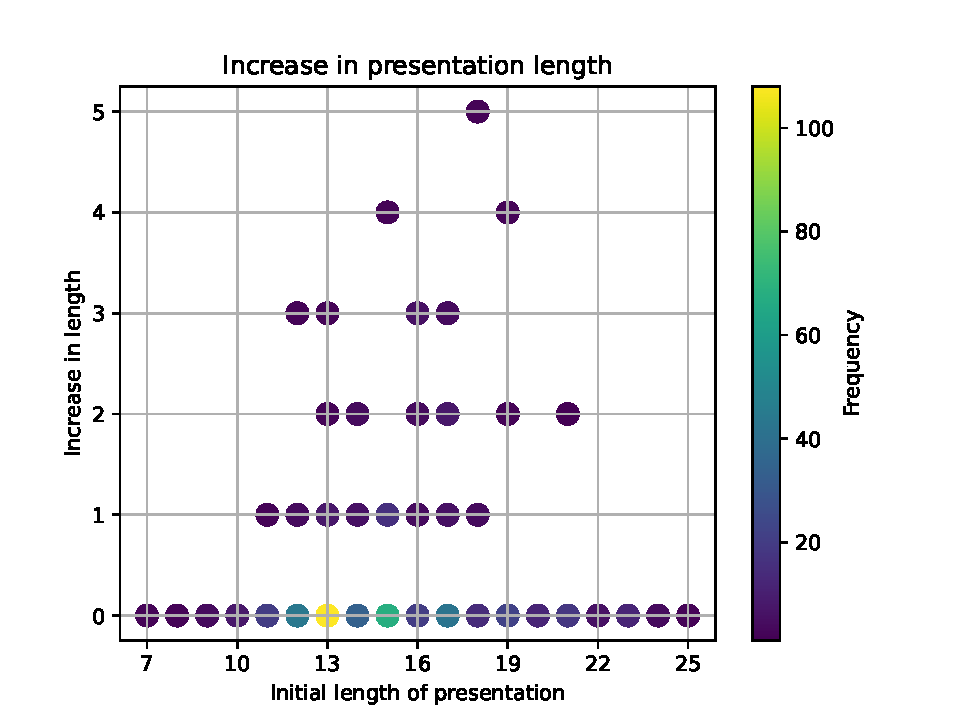
\includegraphics[width=\textwidth]{fig/gs_length_increase_vs_length.pdf}
		\caption{Distribution versus initial presentation length.}
		\label{fig:gs_length_increase_vs_length}
	\end{subfigure}%
	%add desired spacing between images, e. g. ~, \quad, \qquad etc.
	%(or a blank line to force the subfigure onto a new line)
	\begin{subfigure}[b]{0.5\textwidth}
		\centering
		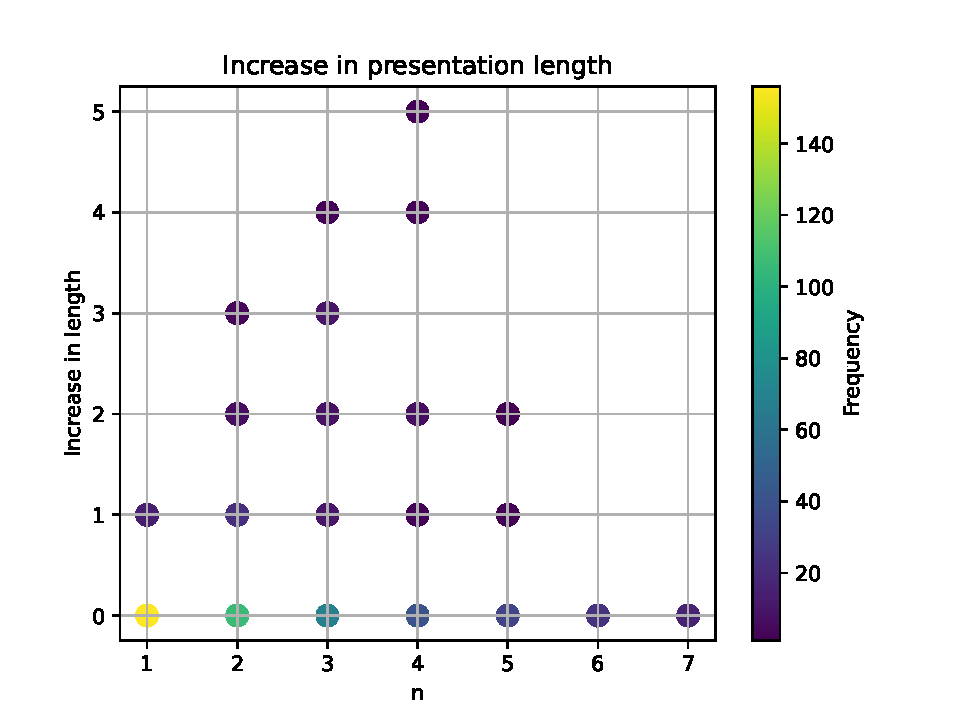
\includegraphics[width=1.1\textwidth]{fig/gs_length_increase_vs_n.pdf}
		\caption{Distribution versus $n$.}
		\label{fig:gs_length_increase_vs_n}
	\end{subfigure}
	\caption{The maximum increase in the length of a presentation relative to its initial length along the AC trivialization path. The increase is plotted as a function of the initial length of the presentation on the left and as a function of $n$ on the right.} \label{fig:gs_length_increase}
\end{figure}

\begin{figure}
	\centering
	\begin{subfigure}[b]{0.4\textwidth}
		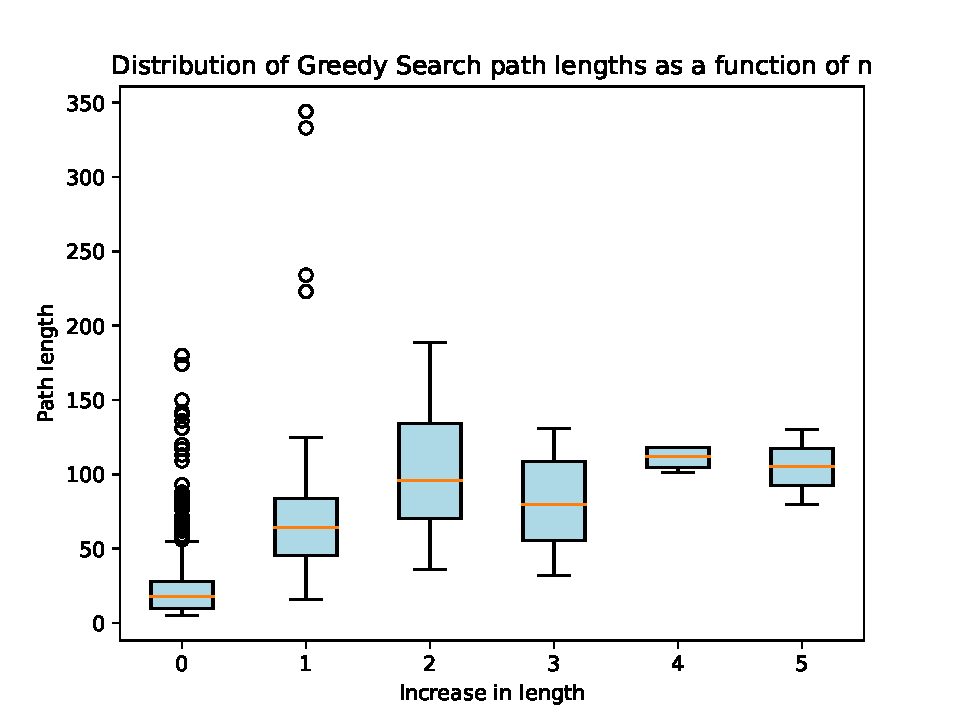
\includegraphics[width=\textwidth]{fig/path_lengths_vs_length_increase.pdf}
		\caption{Distribution versus maximum increase in presentation length.}
		\label{fig:path_lengths_vs_length_increase}
	\end{subfigure}
	\begin{subfigure}[b]{0.4\textwidth}
		\centering
		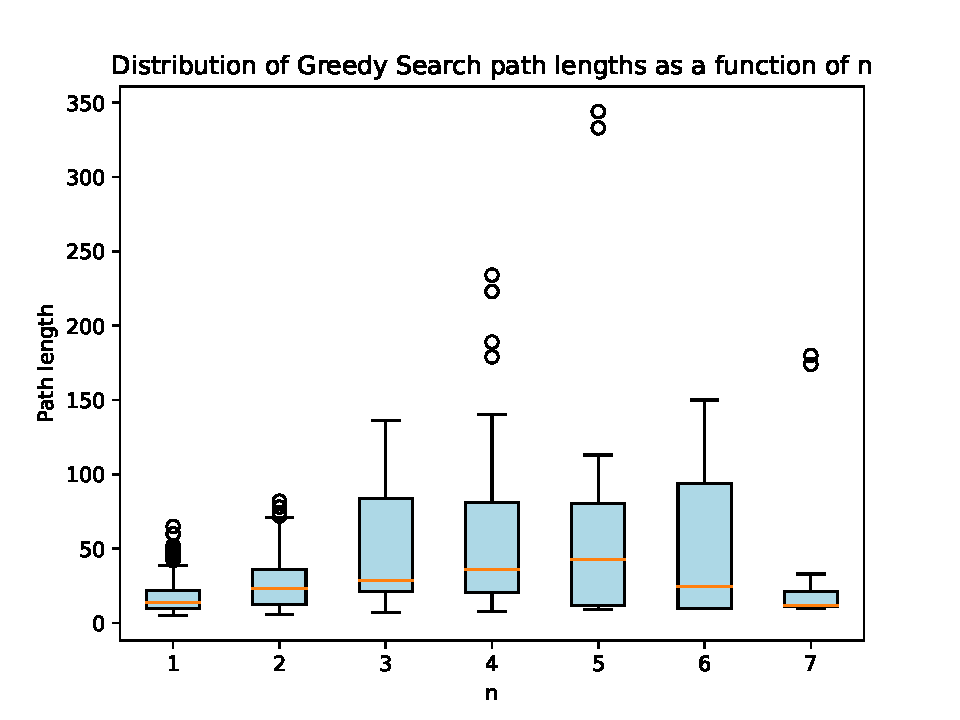
\includegraphics[width=1.1\textwidth]{fig/gs_path_lengths.pdf}
		\caption{Distribution versus $n$.}
		\label{fig:gs_path_lengths}
	\end{subfigure}%
	\caption{Distribution of lengths of AC-trivialization paths learned by greedy search as a function of maximum increase in presentation length (left) and $n$ (right).} \label{fig:gs_path_length}
\end{figure}

\subsection{Limitations}

While the greedy search algorithm performs better than the breadth-first search, it has some of the same limitations.
Namely, it is memory inefficient, and we cannot leverage the parallelizability of modern hardware architectures.
It also does not learn a general algorithm that would find an AC trivialization for any given balanced presentation.

Reinforcement learning algorithms, particularly policy gradient algorithms, present a promising alternative that avoids these downsides.
These algorithms are memory efficient and can be trained in a highly distributed manner, which we will focus on in the next section.

% subsection
% !TEX root = ../ac_paper.tex

\section{Stable AC-trivialization of $\AK(3)$}\label{sec:stable_ak3}

Here we provide a sequence of AC transformations that relates the length-25 stably AC-trivial example of \cite{MMS}, 
\[
\angles{x, y \mid xyx^{-2}y^{-1} xy^{-1}, x^{-1} y^{-1} x y^2 x y^{-1}}.
\]
to $\AK(3)$. We discovered this sequence of transformations using the greedy search algorithm of \autoref{sec:search}. The reader may confirm with the help of a computer program or by hand that this sequence relates the two presentations. To describe the sequence, let us first recall the definitions of AC$'$ moves discussed in \autoref{sec:search},
\begin{enumerate}[label=(AC$'$\arabic*)]
	\item Substitute some $r_i$ by $r_i r_j^{\pm 1}$ for $i \neq j$.
	\item Change some $r_i$ to $g r_i g^{-1}$ where $g$ is a generator or its inverse.
\end{enumerate}

These are 12 transformations, which may be listed as follows.
\[
\begin{aligned}
h_1 &:= \  r_2 \rightarrow r_2 r_1 \\
h_2 &:= \ r_1 \rightarrow r_1 r_2^{-1} \\
h_3 &:= \ r_2 \rightarrow r_2 r_1^{-1} \\
h_4 &:= \ r_1 \rightarrow r_1 r_2 \\
h_5 &:= \ r_2 \rightarrow x^{-1} r_2 x \\
h_6 &:= \ r_1 \rightarrow y^{-1} r_1 y \\
h_7 &:= \ r_2 \rightarrow y^{-1} r_2 y \\
h_8 &:= \ r_1 \rightarrow x r_1 x^{-1} \\
h_9 &:= \ r_2 \rightarrow x r_2 x^{-1} \\
h_{10} &:= \ r_1 \rightarrow y r_1 y^{-1} \\
h_{11} &:= \ r_2 \rightarrow y r_2 y^{-1} \\
h_{12} &:= \ r_1 \rightarrow x^{-1} r_1 x 
\end{aligned}
\]

The sequence of moves that connects the length-25 presentation to $\AK(3)$ is as follows. 
\[
\begin{aligned}
& h_9 \cdot h_7 \cdot h_4 \cdot h_8 \cdot h_{11} \cdot h_5 \cdot h_{11} \cdot h_9 \cdot h_3 \cdot h_{10} \cdot h_{12} \cdot h_7 \cdot h_7 \cdot h_9 \cdot h_{11} \cdot h_5 \cdot h_3 \cdot h_5 \cdot \\
& h_4 \cdot h_3 \cdot h_{12} \cdot h_5 \cdot h_7 \cdot h_7 \cdot h_1 \cdot h_9 \cdot h_{11} \cdot h_8 \cdot h_3 \cdot h_5 \cdot h_{10} \cdot h_2 \cdot h_6 \cdot h_{12} \cdot h_9 \cdot h_7 \cdot \\
& h_5 \cdot h_{11} \cdot h_{10} \cdot h_3 \cdot h_8 \cdot h_{11} \cdot h_9 \cdot h_2 \cdot h_{10} \cdot h_{12} \cdot h_5 \cdot h_7 \cdot h_9 \cdot h_{11} \cdot h_1 \cdot h_9 \cdot h_8
\end{aligned}
\]
This sequence should be read from left to right; first apply $h_9$, then $h_7$, and so forth. This follows the standard convention of many programming languages, which iterate over lists from left to right by default. The total length of the presentation did not exceed $25$ during its path to $\AK(3)$. Additionally, we have not verified if this is the shortest path between the two presentations.



%\[
%\begin{array}{cc}
%[(9, 25), (7, 25), (4, 17), (8, 17), (11, 17), (5, 17), (11, 17), (9, 17), (3, 16), (10, 16), \\
 %(12, 16), (7, 16), (7, 16), (9, 16), (11, 16), (5, 16), (3, 15), (5, 15), (4, 19), (3, 14), (12, 14), \\
 %(5, 14), (7, 16), (7, 18), (1, 19), (9, 19), (11, 19), (8, 19), (3, 18), (5, 18), (10, 18), (2, 15), (6, 15), \\
 %(12, 15), (9, 15), (7, 15), (5, 15), (11, 15), (10, 15), (3, 15), (8, 15), (11, 15), (9, 15), (2, 16),\\
  %(10, 16), (12, 16), (5, 16), (7, 16), (9, 16), (11, 16), (1, 13), (9, 13), (8, 13)]
%\end{array}
%\]

